\documentclass{article}
\usepackage[utf8]{inputenc}
\usepackage[russian]{babel}           
\usepackage[justification=centering]{caption}
\usepackage[backend=bibtex,sorting=none]{biblatex}
\usepackage{fontspec}
\usepackage[final]{graphicx}
\usepackage{tabularx,booktabs}
\newcolumntype{C}{>{\centering\arraybackslash}X} % centered version of "X" type
\setlength{\extrarowheight}{3pt}
\usepackage{float}
\usepackage{subcaption}
\usepackage{mathtools}
\usepackage{adjustbox}
\usepackage{listings}
\usepackage{array}
\usepackage{xcolor}
\usepackage{graphicx}
\usepackage{tikz}
\usepackage{pgfplots}
\usepackage{fontspec}
\usepackage{amssymb}
%\usepackage{unicode-math}
\graphicspath{{./images/}}


\definecolor{codegreen}{rgb}{0,0.6,0}
\definecolor{codegray}{rgb}{0.5,0.5,0.5}
\definecolor{codepurple}{rgb}{0.58,0,0.82}
\definecolor{backcolour}{rgb}{0.95,0.95,0.92}

\newcommand{\A}{\underline{A}}
\newcommand{\B}{\underline{B}}
\newcommand{\und}[1]{\underline{#1}}
\newcommand{\sqft}[3]{#1_{#2}, \ldots, #1_{#3}}

\usepackage[%
        a4paper,%
        includehead,%
        left=2cm,%
        top=0.95cm,%
        right=2cm,%
        bottom=1.65cm,%
        headheight=0.7cm,%
        headsep=0.3cm,%
        footskip=0.8cm]{geometry}
\special{papersize=210mm,297mm}

\lstdefinestyle{mystyle}{
    language=C++,
    backgroundcolor=\color{white},   
    commentstyle=\color{codegreen},
    keywordstyle=[1]{\color{magenta}},
    keywordstyle=[2]{\color{blue}},
    numberstyle=\color{codegray},
    stringstyle=\color{codepurple},
    basicstyle=\ttfamily\footnotesize,
    keywords=[1]{*,<,>,algo, params, param, block, vertex, arg, in},            % if you want to add more keywords to the set
    keywords=[2]{*, id, name, condition, dims, type, val, bsrc, src, value},            % if you want to add more keywords to the set
    breakatwhitespace=false,         
    breaklines=true,                 
    captionpos=b,                    
    keepspaces=true,                 
    numbers=left,                    
    numbersep=10pt,
    xleftmargin=7mm,
    xrightmargin=0mm,
    showspaces=false,                
    showstringspaces=false,
    showtabs=false,                  
    tabsize=4
}
\lstset{style=mystyle}

\lstset{linewidth=1.1\linewidth}
\setmainfont{Times New Roman}
\setmonofont{Monaco}
\title{Отчёт по практическому заданию (3) в рамках курса\\«Суперкомпьютерное моделирование и технологии»\\Вариант 1}
\author{Никифоров Никита Игоревич, гр. 621\\nickiforov.nik@gmail.com}
\date{Октябрь 2022}
\pgfplotsset{compat=1.17}
            
\renewcommand{\baselinestretch}{1.5}
\begin{document}
\maketitle
\newpage
\section{Задача}
    Необходимо реализовать численный метод аппроксимации для трёхмерного 
    гиперболического уравнения в области, представляющей из себя прямоугольный параллелепипед.  
    Для реализации метода предлагается использовать языки программирования 
    {\tt C/C++}, с использованием библиотеки параллельного вычисления {\tt MPI} и {\tt OpenMP}.

    Необходимо провести исследование реализованного численного метода для
    заданного интеграла, области и точности 
    на параллельных вычислительных системах ВМК МГУ: {\tt IBM Polus}
\section{Математическая постановка задачи}
В трёхмерной замкнутой области
\begin{equation*}
    \Omega = [0 \le x \le L_x] \times [0 \le y \le L_y] \times [0 \le z \le L_z]
\end{equation*}
 
Для $(0 < t \le T]$ найти решение $u(x, y, z, t)$ уравнения в частных производных
\begin{equation}
    \frac{\partial^2 u}{\partial t ^ 2} = \Delta u
\end{equation}
 
С начальными условиями 
\begin{equation}
    u \rvert_{t = 0} = \varphi (x, y, z)
    \label{eq:phi}
\end{equation}
\begin{equation}
    \frac{\partial u}{\partial t} \bigg \rvert_{t=0} = 0
\end{equation}
 
Граничные условия (вариант 1):
\begin{align}
    u(0, y, z, t) &= 0 && u(L_x, y, z, t) = 0\\ 
    u(x, 0, z, t) &= 0 && u(x, L_y, z, t) = 0\\
    u(x, y, 0, t) &= 0 && u(x, y, L_z, t) = 0
\end{align}
 
Аналитическое решение:
\begin{align}
    & u_{analytical}(x, y, z, t) = sin(\frac{\pi}{L_x}x) \cdot sin(\frac{2\pi}{L_y}y) \cdot sin(\frac{3\pi}{L_z}z) \cdot cos(a_y \cdot t), \\
    & a_t = \sqrt{\frac{1}{L_x^2} + \frac{4}{L_y^2} + \frac{9}{L_z^2}}
\end{align}
 
\section*{Численный метод решения задачи}
Для решения введём на $\Omega$ сетку $\omega_{h \tau} = \bar{\omega}_h \times \omega_{\tau}$
\begin{align*}
    &\bar{\omega}_h = \{(x_i = ih_x, y_i = jh_y, z_k = kh_z), i, j, k = 0, ..., N, h_x N = L_x, h_y N = L_y, h_z N = L_z\}\\
    &\omega_{\tau} = \{t_n = n\tau n = 0, 1, ..., K, \tau K = T\}
\end{align*}
 
Для аппроксимации уравнения воспользуемся равенством:
\begin{equation}
    \frac{u_{ijk}^{n+1} - 2 u_{ijk}^n + u_{ijk}^{n - 1}}{\tau^2} = \Delta_h u^n 
\end{equation}
\begin{align}
    \Delta_h u^n &= \frac{u_{i-1,j,k}^n - 2 u_{i,j,k}^n + u_{i+1,j,k}^n}{h^2} + \frac{u_{i,j-1,k}^n - 2 u_{i,j,k}^n + u_{i,j+1,k}^n}{h^2} +\\
    &+ \frac{u_{i,j,k-1}^n - 2 u_{i,j,k}^n + u_{i,j,k+1}^n}{h^2}
\end{align}
 
(Если $L_x = L_y = L_z$, то $h_x = h_y = h_z = h$).
 
Для начала счёта находим $u^0$. Из условия (\ref{eq:phi}) получаем:
\begin{equation}
    u_{ijk}^0 = \varphi (x_i, y_j, z_k), \quad (x_i, y_j, z_k) \in \omega_h.
\end{equation}
 
Следующий шаг:
\begin{equation}
    \frac{u_{ijk}^1 - u_{ijk}^0}{\tau} = \frac{\tau}{2}\Delta_h \varphi (x_i, y_j, z_k) \quad (x_i, y_j, z_k) \in \omega_h
\end{equation}
\begin{equation}
    u_{ijk}^1 = u_{ijk}^0 + \frac{\tau ^ 2}{2} \Delta_h \varphi (x_i, y_j, z_k)
\end{equation}

\section{Аналитическое решение задачи}
    \begin{equation}
        \varphi (x, y, z, t) = sin(\frac{\pi * x}{L_x})sin(\frac{\pi * y}{L_y})sin(\frac{\pi * z}{L_z})cos(a_t * t)
    \end{equation}
\section{Программная реализация}
    \subsection{MPI}
    Для программной реализации предложенного метода используется язык {\tt C++}, а также 
    библиотека параллельного программирования {\tt MPI} и {\tt OpenMP}.
    
    Для эффективной программной реализации предложенного численного метода
    предлагается разбить вычисления на трёхмерную сетку, каждый блок
    из которых вычисляется на своём {\tt MPI} процессе. Для создания топологии процессов
    используются функции библиотеки {\tt MPI}: 
    \begin{itemize}
        \item {\tt MPI\_Dims\_create}~--- для автоматического получения размерностей сетки процессов,
        \item {\tt MPI\_Cart\_create}~--- для создания сетки процессов {\tt MPI}.
    \end{itemize}

    В качестве аргументов функция {\tt MPI\_Dims\_create} принимает количество процессов {\tt MPI},
    а возвращает сбалансированную размерность сетки процессов.

    В качестве аргументов функция {\tt MPI\_Cart\_create} принимает размерность стеки,
    периодичность граней, а также необходимость размещать близкие по сетке на близких 
    физических ядрах.

    В каждом {\tt MPI} процессе выполняется следующий алгоритм:
    \begin{enumerate}
        \item Вычислить в блоке значения в точках сетки по формулам (8) и (9).
        \item Вычислить ошибку аппроксимации как \(max_{i, j, k}(|u^n_{xyz} - analitical_solution(x, y, z, t)|)\).
        \item Скопировать грани вычисленного блока в непрерывные буферы.
        \item Провести обмены с соседними блоками непрерывными буферами.
    \end{enumerate}
\begin{lstlisting}
void calc_next() {
    for (int i = start[0]; i < bsize[0] - end[0]; i++) {
        for (int j = start[1]; j < bsize[1] - end[1]; j++) {
            for (int k = start[2]; k < bsize[2] - end[2]; k++) {
                double lap = func_lap(i, j, k, *data[1]);
                (*data[2])(i, j, k) = tau*tau*lap + 2 * (*data[1])(i, j, k) - 
                                      (*data[0])(i, j, k);
            }
        }
    } 
}
\end{lstlisting}

    Из особенностей реализации можно указать необходимость отслеживать глобальные координаты
    в каждом блоке, так как внутри блока адресация идёт в относительных координатах,
    поэтому при вызове аналитической функции идёт смешение относительных координат, для
    получения глобальных координат в сетке.

\subsection{OpenMP}
    Для использования библиотеки {\tt OpenMP} перед каждым циклом прописывается 
    директива {\tt \#pragma omp parallel for collapse(N) num\_threads(THREADS)}, где:
    \begin{itemize}
        \item {\tt \#pragma omp parallel for}~--- основная часть директивы, которая
            говорит компилятору, где находится цикл, вычисление которого необходимо 
            исполнить на нескольких потоках.
        \item {\tt collapse(N)}~--- указывает вложенность циклов, где {\tt N}, уровень
            вложенности цикла.
        \item {\tt num\_threads(THREADS)}~--- указывает количество потоков, которое необходимо
            использовать. Здесь {\tt THREADS = 4}.
    \end{itemize}

    При подсчёте ошибки используется дополнительно директива редукции {\tt reduction(max:error)}
    
\section{Исследование программной реализации}
    Для исследования использовалась система Polus и домашний компьютер.
    Характеристики узла системы параллельного вычисления Polus (на данный момент имеет в работе 3 узла):
    \begin{itemize}
        \item 2 десятиядерных процессора IBM POWER8 (каждое ядро имеет 8 потоков) всего 160 потоков
        \item Общая оперативная память 256 Гбайт (в узле 5 оперативная память 1024 Гбайт) с ЕСС контролем
        \item 2 х 1 ТБ 2.5” 7K RPM SATA HDD
        \item 2 x NVIDIA Tesla P100 GPU, 16Gb, NVLink
        \item 1 порт 100 ГБ/сек
    \end{itemize}

    %Характеристики домашнего PC:
    %\begin{itemize}
    %    \item 1 шестнадцати ядерный процессор AMD Ryzen 5950X, всего 32 потока на частоте 4.4Ghz
    %    \item Оперативная память 32 Гбайт
    %    \item SSD NVMe Samsung 500 ГБ
    %    \item AMD RX 5600XT
    %\end{itemize}

    Необходимо провести экспериментальное исследование для \(L_x = L_y = L_z = 1\) и \(L_x = L_y = L_z = \pi\).
    И для разного количества процессов для MPI версии: \(cpus = 1, 4, 8, 16, 32\), для OpenMP+MPI: \(cpus = 1, 2, 4, 8\).
    И для различного числа точек в сетке \(128^3, 256^3, 512^3\).

    Ускорение считалось как отношение общего времени выполнения 
    на одном MPI-процессе ко времени вычисления на заданном количестве MPI-процессов.
    Составим таблицу для системы Polus:
    \begin{table*}[!t]
        \centering
        \caption{Результаты исследования на машине Polus \(L_x = L_y = L_z = 1\)}\label{tab:tab1}
        \begin{tabularx}{\textwidth}{@{}l*{10}{C}c@{}} %{|m{3.5cm}|m{2.5cm}|m{2cm}|m{3.5cm}|m{4cm}|}
            \toprule
            \bf Размер сетки & \bf число MPI процессов  & \bf Время работы (с) & \bf Ускорение по времени & \bf Ошибка \\
                \midrule
                \(128*128*128\) & 1  & 2.356270 & 1     & 3.32669e-09\\
                \(128*128*128\) & 4  & 0.630888 & 3.73  & 3.32669e-09\\
                \(128*128*128\) & 8  & 0.457156 & 5.15  & 3.32669e-09\\
                \(128*128*128\) & 16 & 0.402237 & 5.85  & 3.32669e-09\\
                \(128*128*128\) & 32 & 0.194718 & 12.10 & 3.32669e-09\\
                \midrule
                \(256*256*256\) & 1  & 18.57330 & 1     & 8.24106e-10 \\
                \(256*256*256\) & 4  & 4.704710 & 3.94  & 8.24106e-10 \\
                \(256*256*256\) & 8  & 2.840980 & 6.53  & 8.24106e-10 \\
                \(256*256*256\) & 16 & 1.571960 & 11.81 & 8.24106e-10 \\
                \(256*256*256\) & 32 & 0.890774 & 20.85 & 8.24106e-10 \\
                \midrule
                \(512*512*512\) & 1  & 150.018 & 1      & 2.04022e-10 \\
                \(512*512*512\) & 4  & 37.8112 & 3.96   & 2.04022e-10 \\
                \(512*512*512\) & 8  & 20.2954 & 7.39   & 2.04022e-10 \\
                \(512*512*512\) & 16 & 10.7692 & 13.93  & 2.04022e-10 \\
                \(512*512*512\) & 32 & 5.54698 & 27.04  & 2.04022e-10 \\
                \bottomrule
            \end{tabularx}
        \end{table*}
       \begin{table*}[!t]
        \centering
        \caption{Результаты исследования на машине Polus \(L_x = L_y = L_z = \pi\)}\label{tab:tab1}
        \begin{tabularx}{\textwidth}{@{}l*{10}{C}c@{}} %{|m{3.5cm}|m{2.5cm}|m{2cm}|m{3.5cm}|m{4cm}|}
            \toprule
            \bf Размер сетки & \bf число MPI процессов  & \bf Время работы (с) & \bf Ускорение по времени & \bf Ошибка \\
                \midrule
                \(128*128*128\) & 1  & 2.097480 & 1     & 0.00423684\\
                \(128*128*128\) & 4  & 0.529625 & 3.96  & 0.00423684\\
                \(128*128*128\) & 8  & 0.319248 & 6.57  & 0.00423684\\
                \(128*128*128\) & 16 & 0.325514 & 6.44  & 0.00423684\\
                \(128*128*128\) & 32 & 0.259678 & 8.07  & 0.00423684\\
                \midrule
                \(256*256*256\) & 1  & 16.13620 & 1     & 0.0170563 \\
                \(256*256*256\) & 4  & 4.044850 & 3.98  & 0.0170563 \\
                \(256*256*256\) & 8  & 2.386630 & 6.76  & 0.0170563 \\
                \(256*256*256\) & 16 & 1.240480 & 13.00 & 0.0170563 \\
                \(256*256*256\) & 32 & 0.715582 & 22.54 & 0.0170563 \\
                \midrule
                \(512*512*512\) & 1  & 130.179 & 1      & 0.0667194 \\
                \(512*512*512\) & 4  & 32.7986 & 3.96   & 0.0667194 \\
                \(512*512*512\) & 8  & 16.7369 & 7.77   & 0.0667194 \\
                \(512*512*512\) & 16 & 8.91785 & 14.59  & 0.0667194 \\
                \(512*512*512\) & 32 & 4.58811 & 28.37  & 0.0667194 \\
                \bottomrule
            \end{tabularx}
        \end{table*}
        \begin{table*}[!t]
        \centering
        \caption{Результаты исследования на домашнем ПК \(L_x = L_y = L_z = 1\)}\label{tab:tab1}
        \begin{tabularx}{\textwidth}{@{}l*{10}{C}c@{}} %{|m{3.5cm}|m{2.5cm}|m{2cm}|m{3.5cm}|m{4cm}|}
            \toprule
            \bf Размер сетки & \bf число MPI процессов  & \bf Время работы (с) & \bf Ускорение по времени & \bf Ошибка \\
                \midrule
                \(128*128*128\) & 1 & 1.7638   & 1     & 3.32669e-09\\
                \(128*128*128\) & 2 & 0.284199 & 6.20  & 3.32669e-09\\
                \(128*128*128\) & 4 & 0.16448  & 10.72 & 3.32669e-09\\
                \(128*128*128\) & 8 & 0.099784 & 17.67 & 3.32669e-09\\
                \midrule
                \(256*256*256\) & 1 & 11.6942 & 1     & 8.24106e-10 \\
                \(256*256*256\) & 2 & 2.20329 & 5.30  & 8.24106e-10 \\
                \(256*256*256\) & 4 & 1.12874 & 10.36 & 8.24106e-10 \\
                \(256*256*256\) & 8 & 0.59743 & 19.57 & 8.24106e-10 \\
                \midrule
                \(512*512*512\) & 1 & 40.15   & 1      & 2.04022e-10 \\
                \(512*512*512\) & 2 & 17.6784 & 2.27   & 2.04022e-10 \\
                \(512*512*512\) & 4 & 9.06548 & 4.42   & 2.04022e-10 \\
                \(512*512*512\) & 8 & 4.69384 & 8.55   & 2.04022e-10 \\
                \bottomrule
            \end{tabularx}
        \end{table*}
       \begin{table*}[!t]
        \centering
        \caption{Результаты исследования на машине Polus \(L_x = L_y = L_z = \pi\)}\label{tab:tab1}
        \begin{tabularx}{\textwidth}{@{}l*{10}{C}c@{}} %{|m{3.5cm}|m{2.5cm}|m{2cm}|m{3.5cm}|m{4cm}|}
            \toprule
            \bf Размер сетки & \bf число MPI процессов  & \bf Время работы (с) & \bf Ускорение по времени & \bf Ошибка \\
                \midrule
                \(128*128*128\) & 1 & 1.85292  & 1     & 0.00423684\\
                \(128*128*128\) & 2 & 0.280265 & 6.61  & 0.00423684\\
                \(128*128*128\) & 4 & 0.159591 & 11.61  & 0.00423684\\
                \(128*128*128\) & 8 & 0.095655 & 19.37  & 0.00423684\\
                \midrule
                \(256*256*256\) & 1 & 10.8742 & 1     & 0.0170563 \\
                \(256*256*256\) & 2 & 2.15846 & 5.03  & 0.0170563 \\
                \(256*256*256\) & 4 & 1.09877 & 9.89  & 0.0170563 \\
                \(256*256*256\) & 8 & 0.58233 & 18.67 & 0.0170563 \\
                \midrule
                \(512*512*512\) & 1 & 33.6420 & 1      & 0.0667194 \\
                \(512*512*512\) & 2 & 17.3213 & 1.94   & 0.0667194 \\
                \(512*512*512\) & 4 & 8.68217 & 3.87   & 0.0667194 \\
                \(512*512*512\) & 8 & 4.40099 & 7.64   & 0.0667194 \\
                \bottomrule
            \end{tabularx}
        \end{table*}
        \clearpage

\begin{figure*}[!t]
\centering
    \includegraphics[width=\textwidth,trim=0 0 0 0,clip]{an_sol_hm.pdf}
    \caption{График аналитического решения \(time = 0\), \(L_x=L_y = L_z = 1\), сетка \(10^3\).}
    \label{img:1}
\end{figure*}

\begin{figure*}[!t]
\centering
    \includegraphics[width=\textwidth,trim=0 0 0 0,clip]{calc_sol_hm.pdf}
    \caption{График посчитанного решения \(time = 21\), \(L_x = L_y = L_z = 1\), сетка \(10^3\).}
    \label{img:2}
\end{figure*}


\begin{figure*}[!t]
\centering
    \includegraphics[width=\textwidth,trim=0 0 0 0,clip]{calc_sol_err_hm.pdf}
    \caption{График погрешности решения \(time = 21\), \(L_x = L_y = L_z = 1\), сетка \(10^3\).}
    \label{img:3}
\end{figure*}

\begin{figure*}[!t]
\centering
\begin{subfigure}[b]{0.49\textwidth}
    \centering
    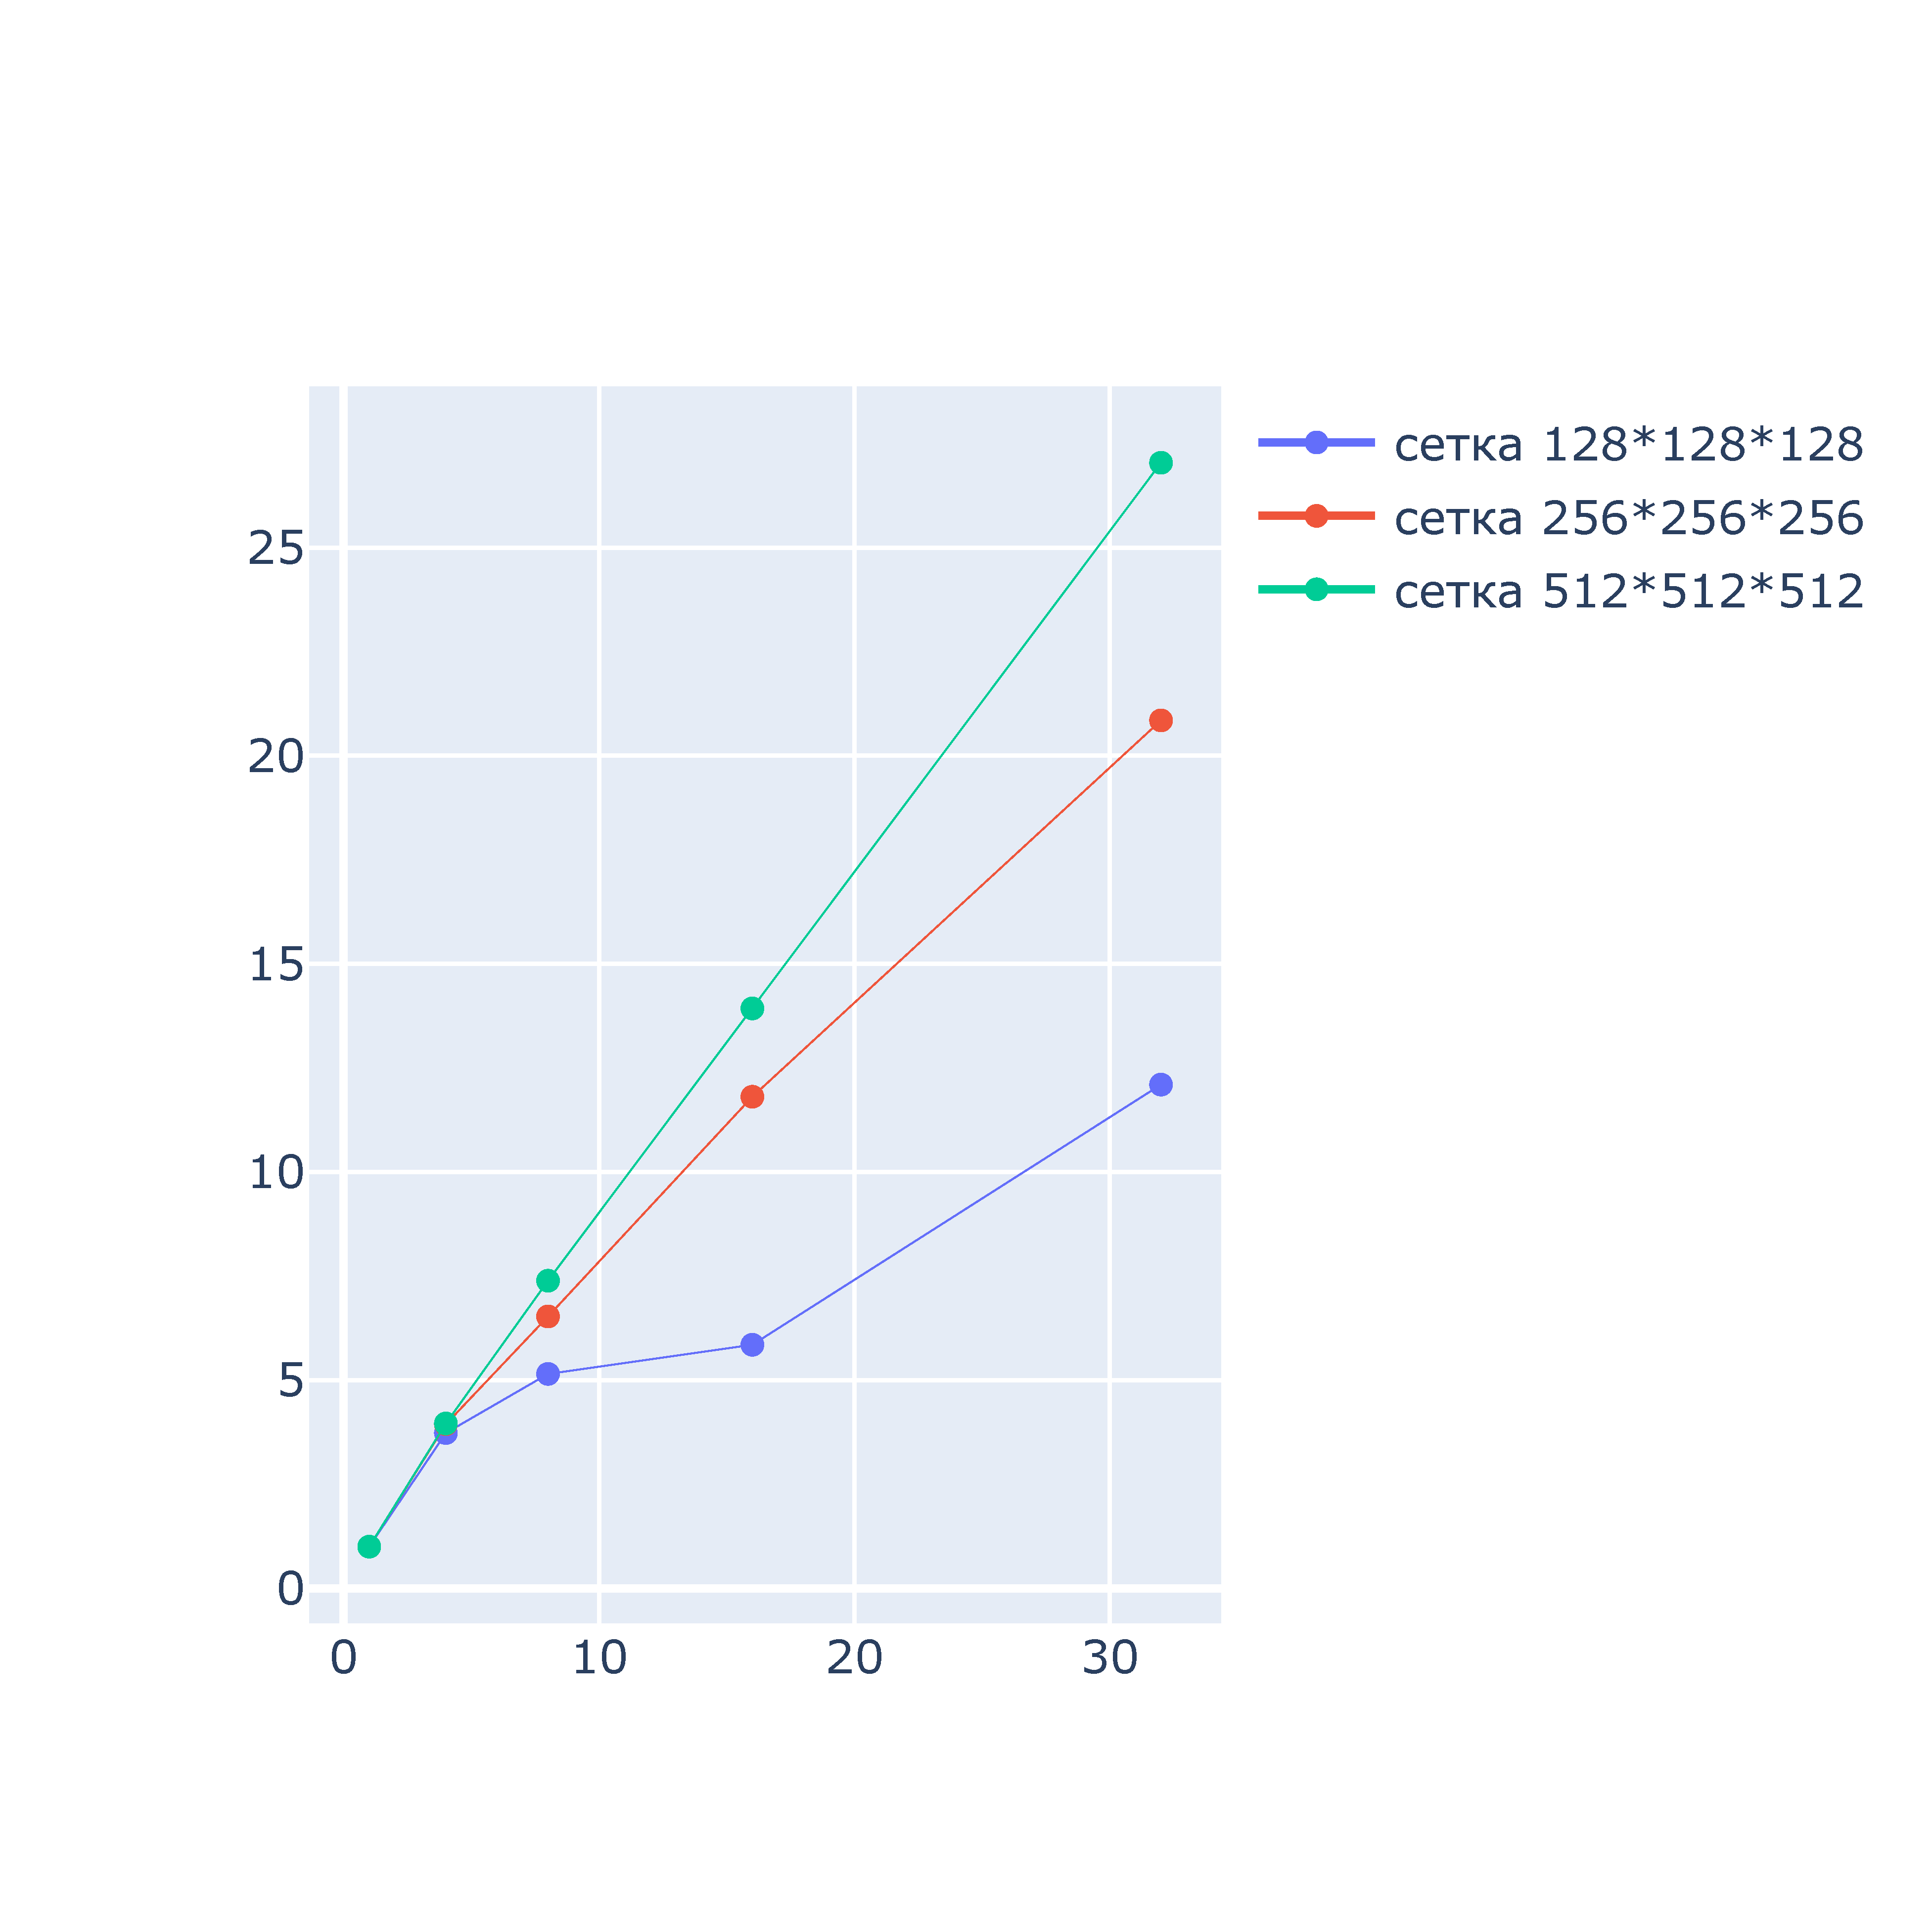
\includegraphics[width=\textwidth,trim=0 0 0 0,clip]{mpi_l_0.pdf}
    \caption{\(L_x=L_y=L_z=1\)}
    \label{img:1.1}
\end{subfigure}
\begin{subfigure}[b]{0.49\textwidth}
    \centering
    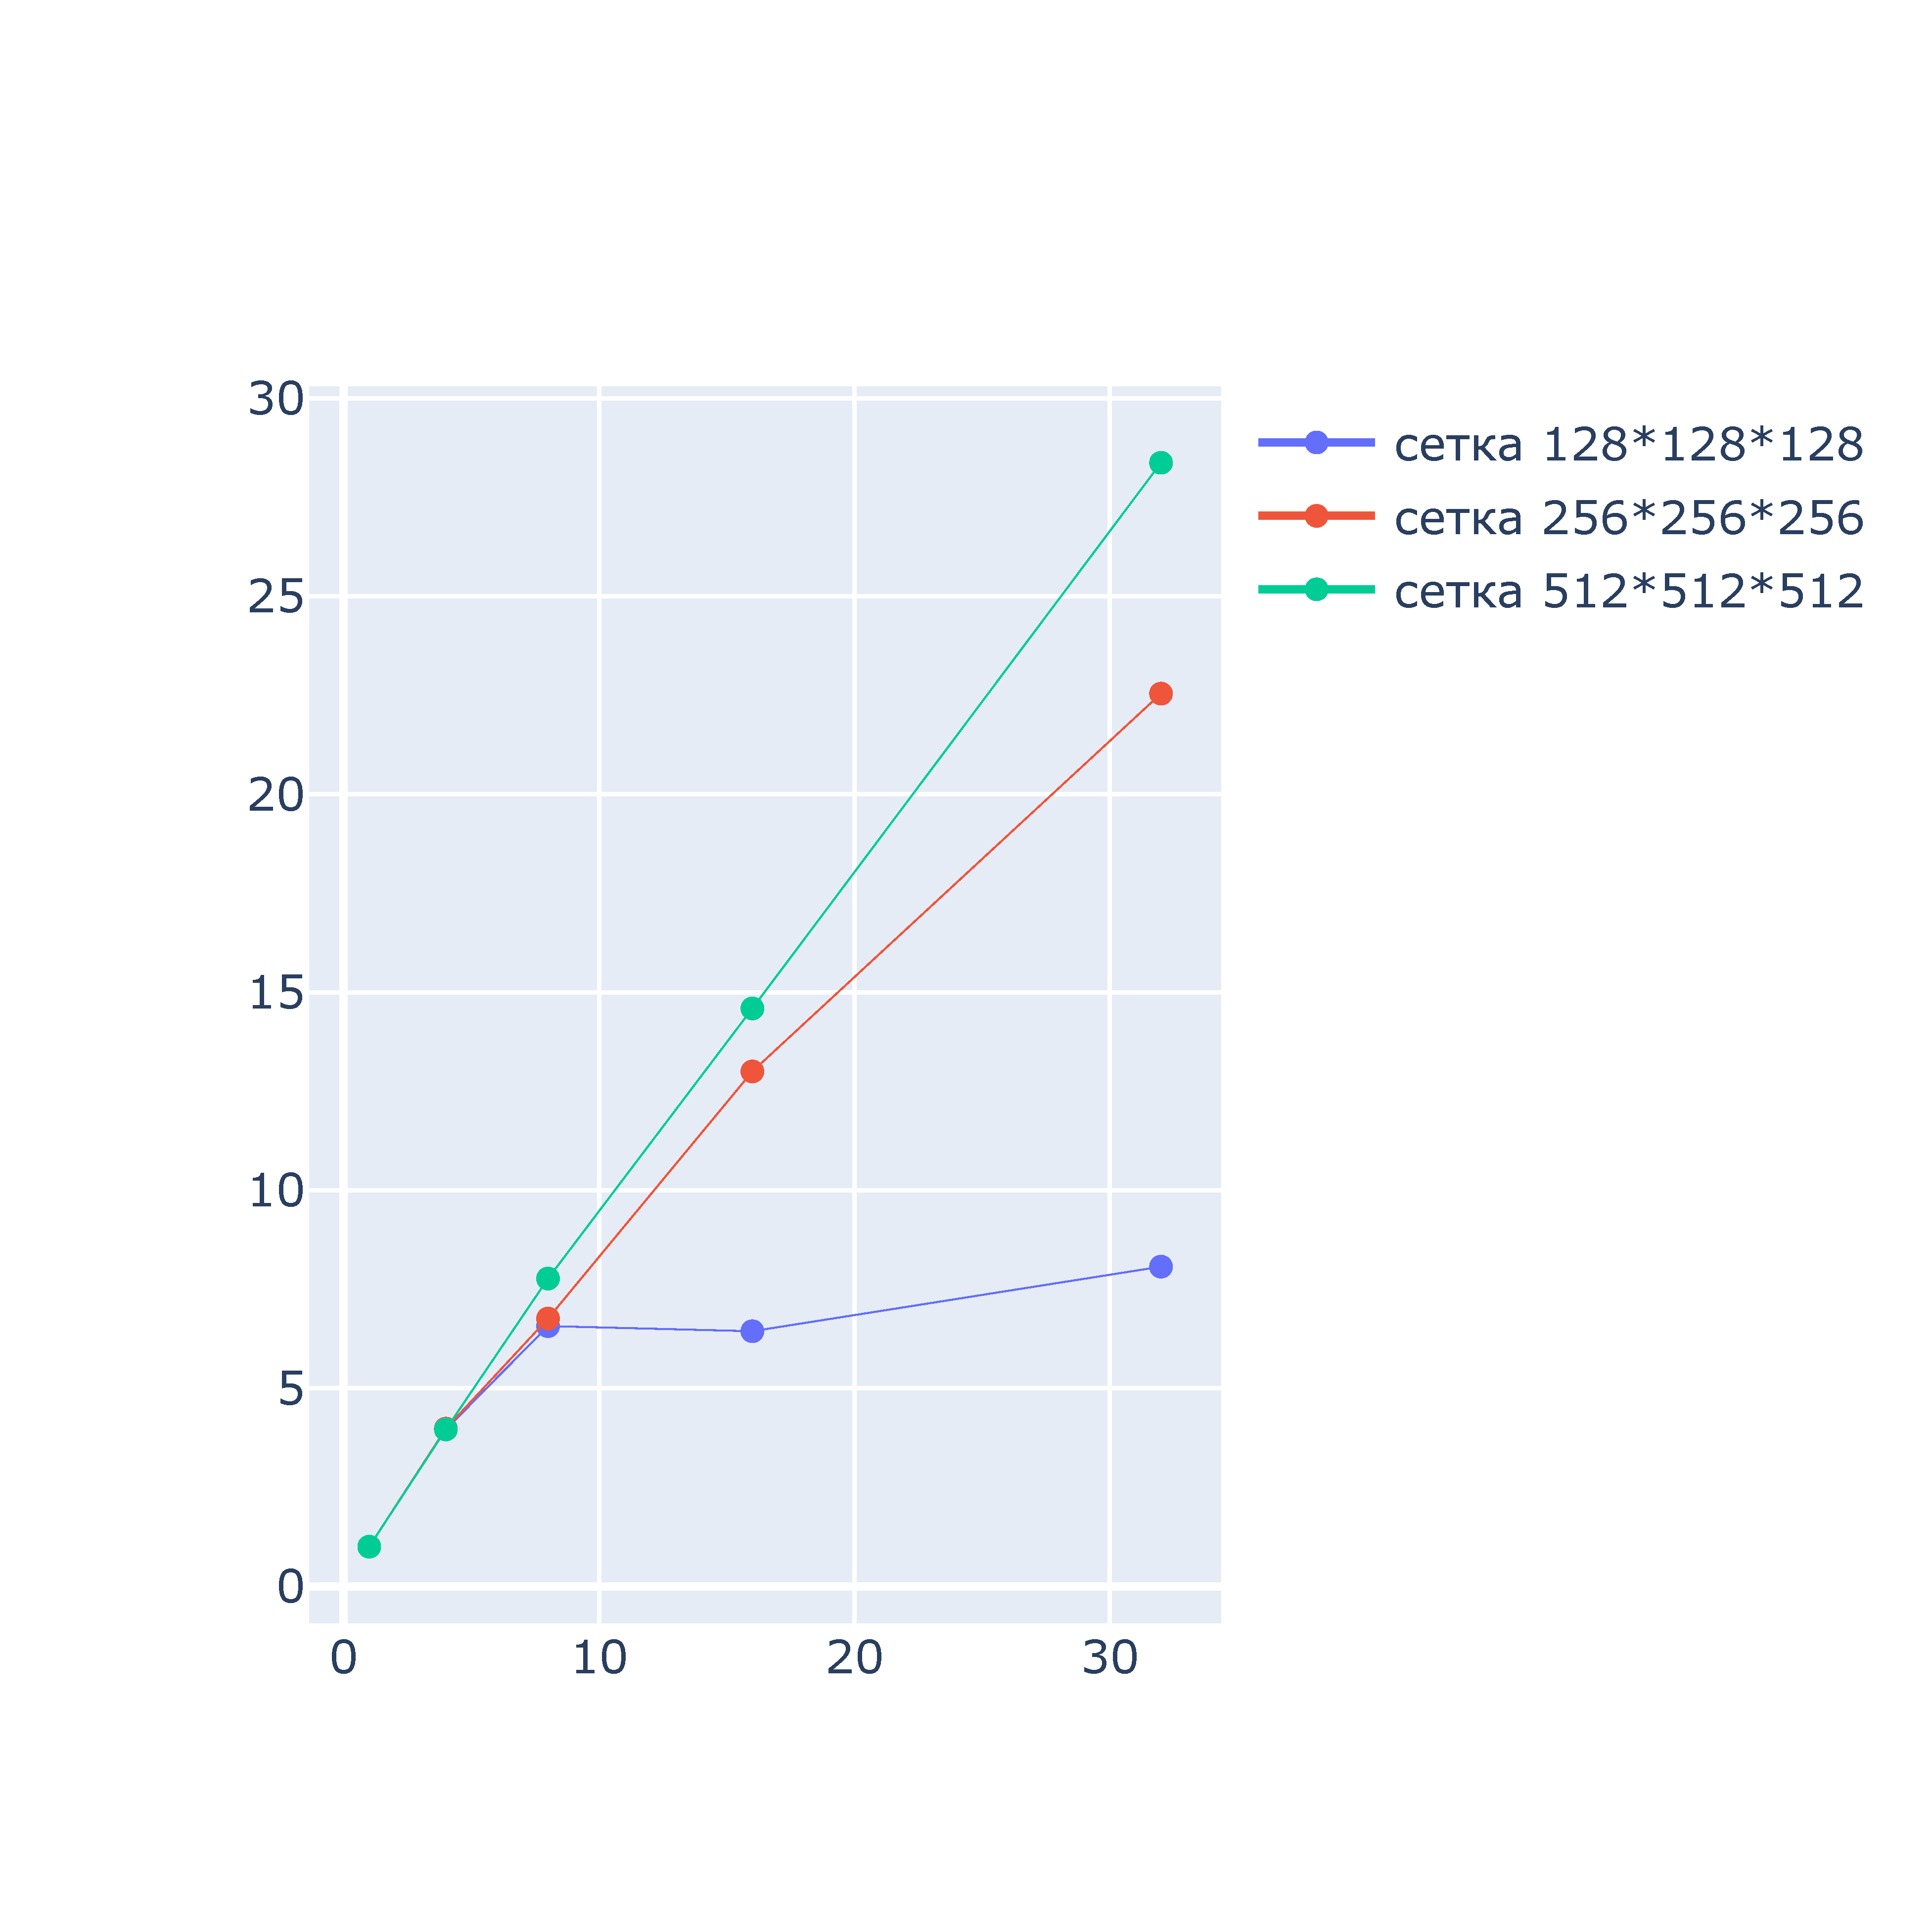
\includegraphics[width=\textwidth,trim=0 0 0 0,clip]{mpi_l_1.pdf}
    \caption{\(L_x=L_y=L_z=\pi\)}
    \label{img:1.2}
\end{subfigure}
\caption{График зависимости ускорения от числа процессов MPI, на различных сетках}
\end{figure*}

\begin{figure*}[!t]
\centering
\begin{subfigure}[b]{0.49\textwidth}
    \centering
    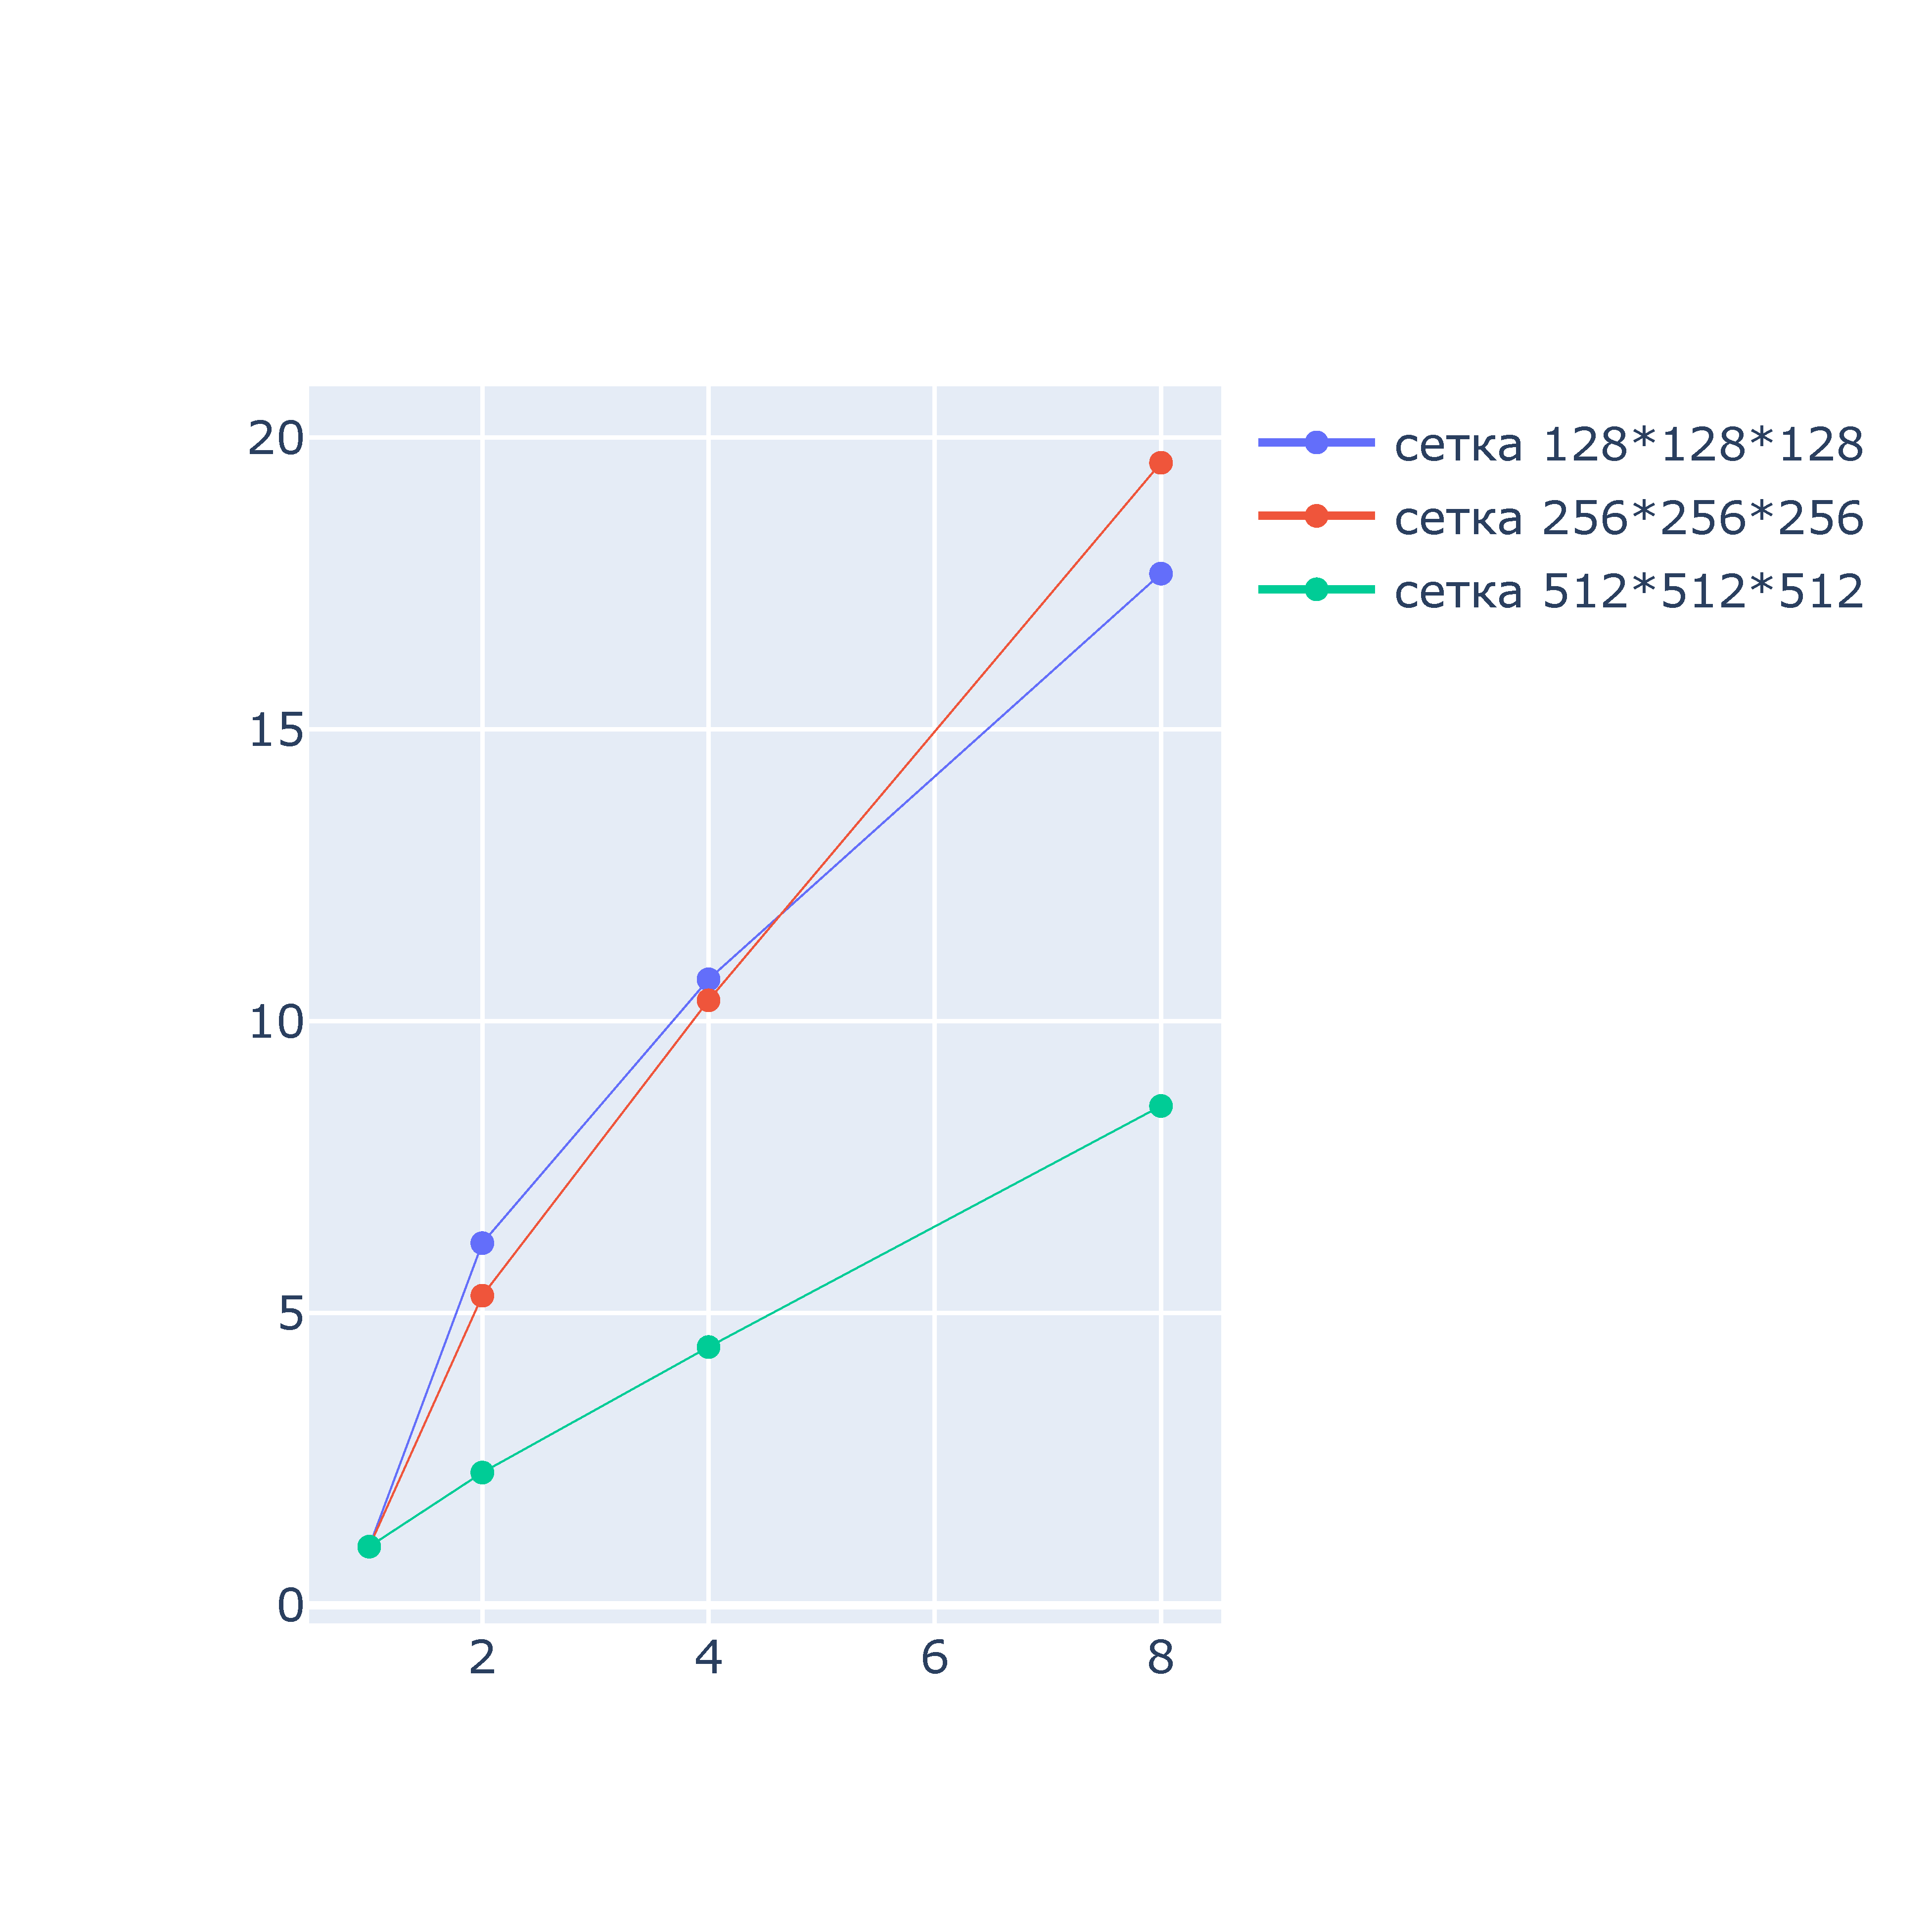
\includegraphics[width=\textwidth,trim=0 0 0 0,clip]{omp_l_0.pdf}
    \caption{\(L_x=L_y=L_z=1\)}
    \label{img:1.1}
\end{subfigure}
\begin{subfigure}[b]{0.49\textwidth}
    \centering
    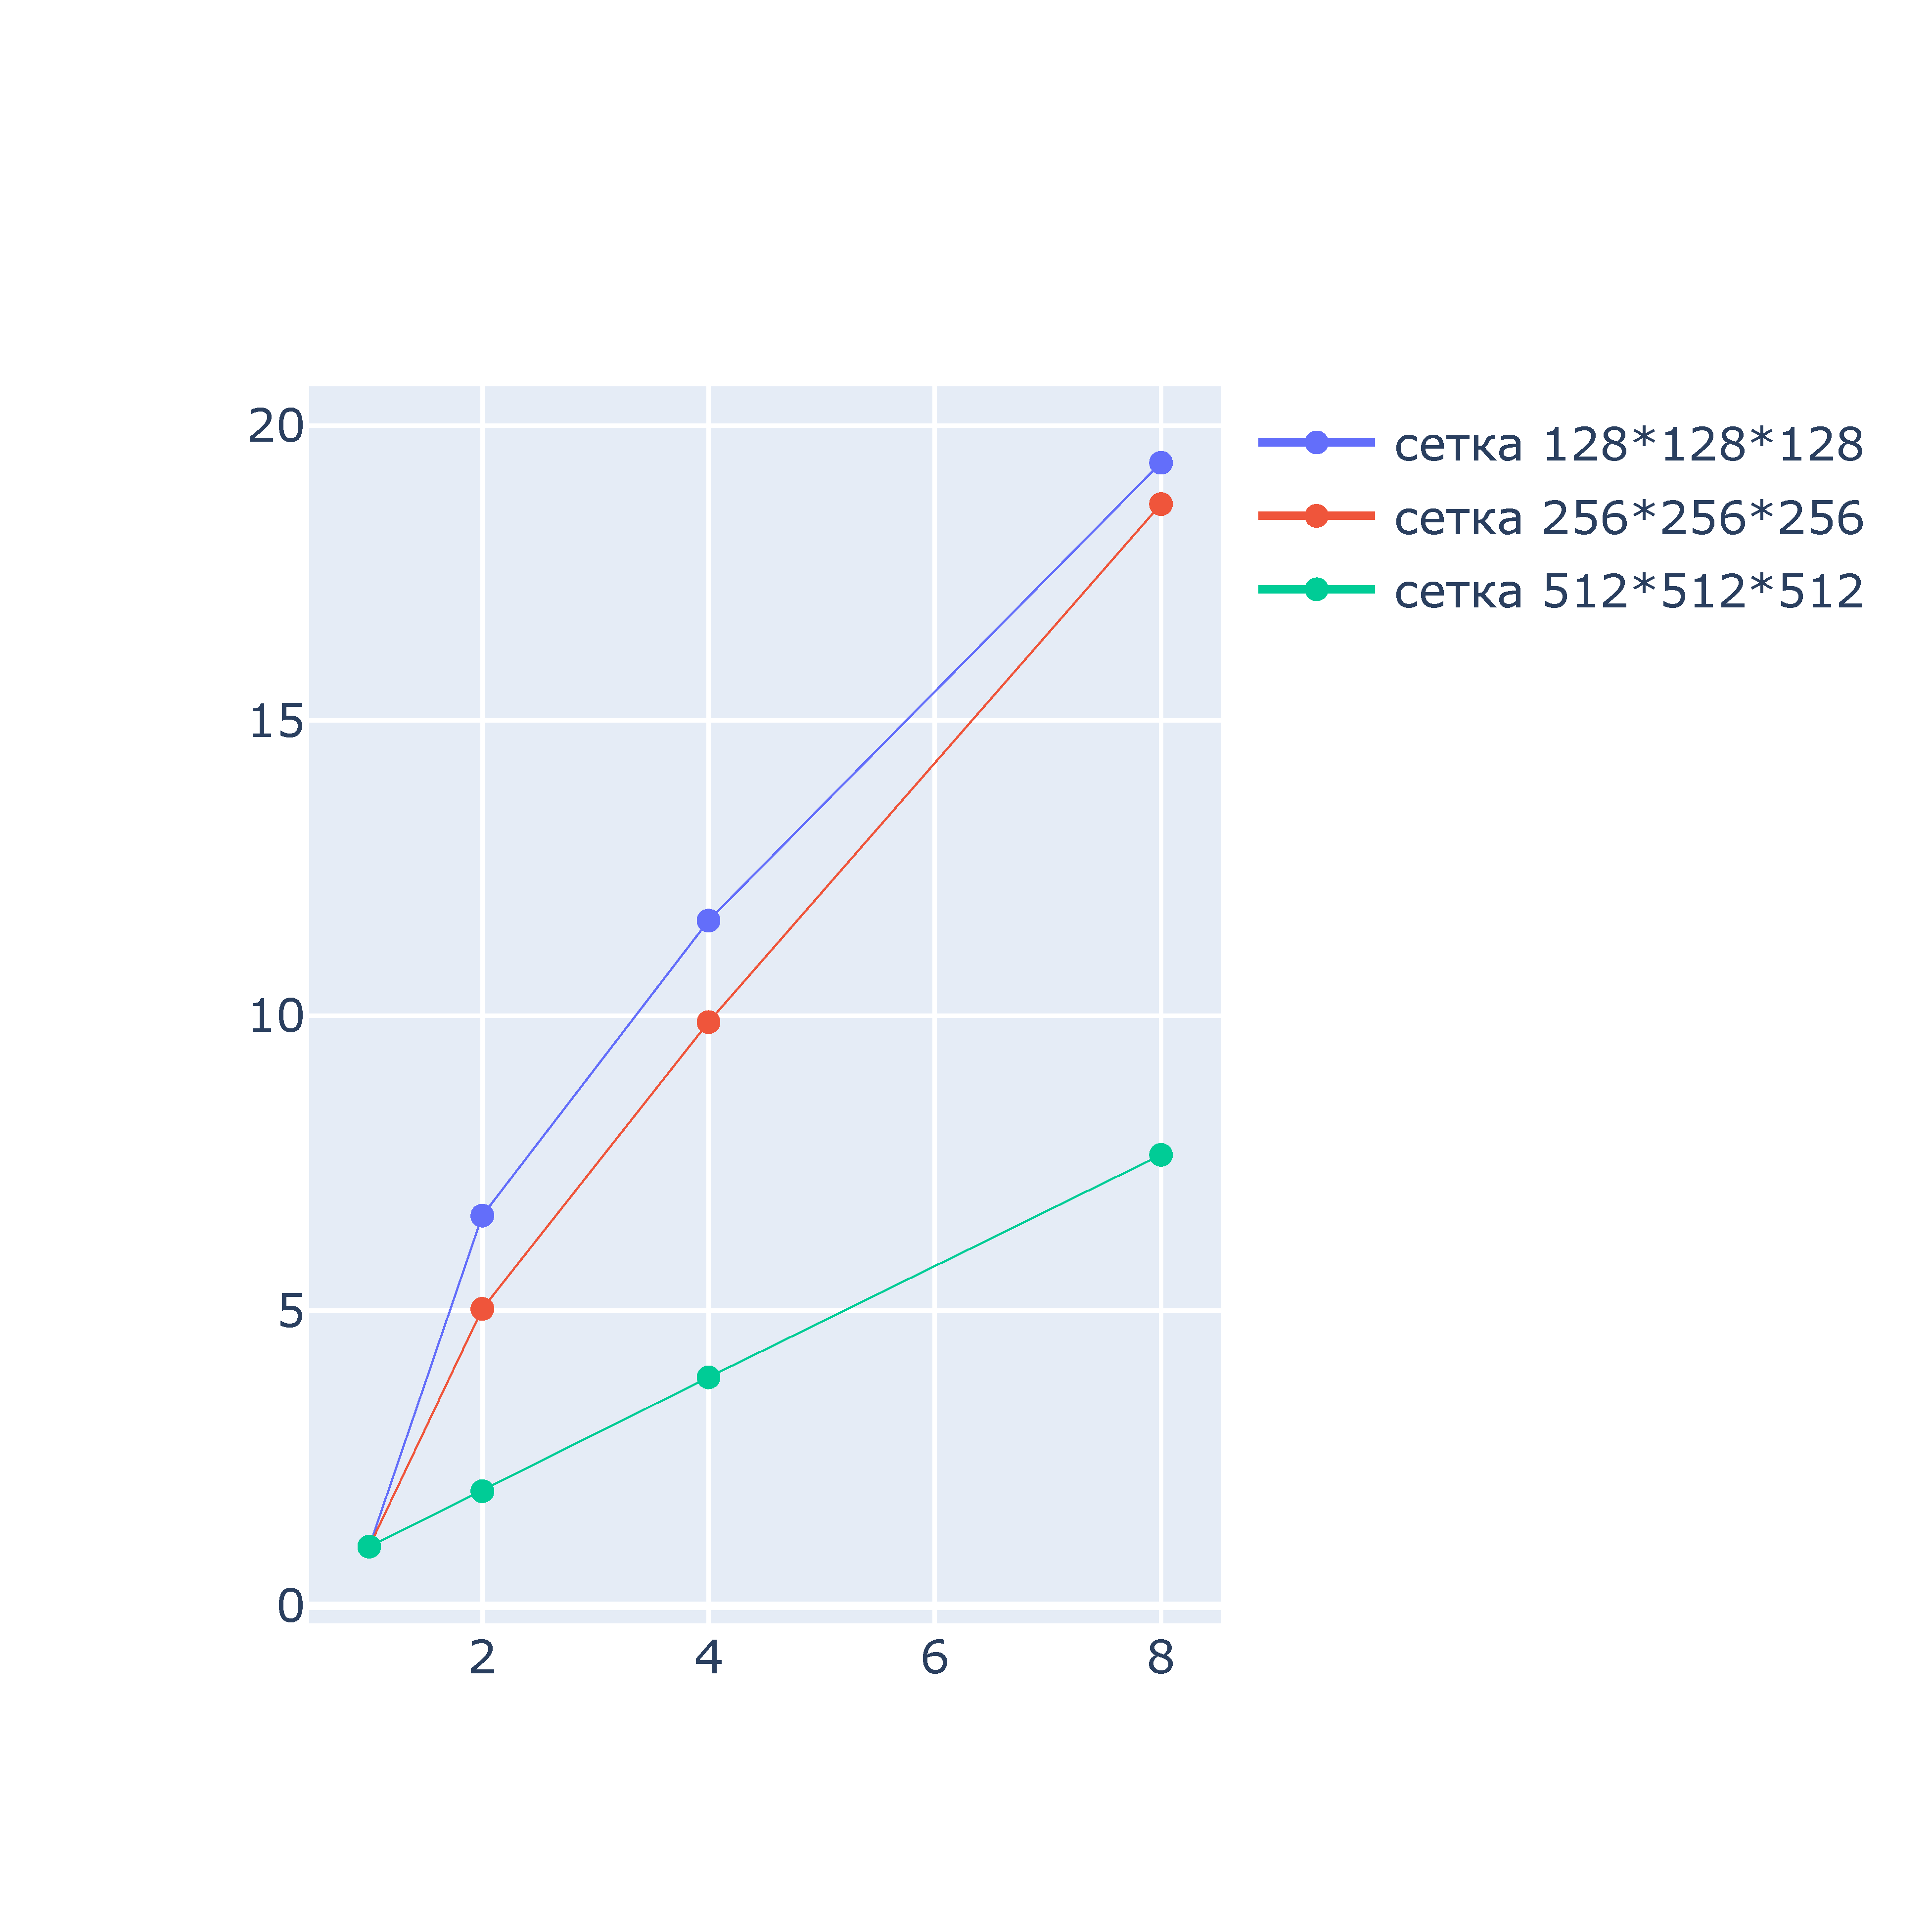
\includegraphics[width=\textwidth,trim=0 0 0 0,clip]{omp_l_1.pdf}
    \caption{\(L_x=L_y=L_z=\pi\)}
    \label{img:1.2}
\end{subfigure}
\caption{График зависимости ускорения от числа процессов MPI, реализация MPI+OpenMP, на различных сетках}
\end{figure*}
\end{document}
